\section {Вычисления на графических процессорах}

В немалой степени развитию параллельных вычислений на графических процессорах способствовали компьютерные игры. Устройства для параллельных векторных вычислений, которые часто применяются в 3D графике, достигают очень высокой производительности, недоступной для универсальных процессоров. Вслед за первыми видеокартами с поддержкой параллельных вычислений возникли технологии неграфических расчётов общего назначения GPGPU (General Purpose computation on GPUs). Современные видеочипы содержат сотни математических исполнительных блоков, и эта мощь может использоваться для значительного ускорения множества вычислительно-интенсивных приложений. Разработчики задумали сделать так, чтобы GPU рассчитывали не только изображение в 3D приложениях, но и применялись в других параллельных расчётах.

В дальнейшем, два основных производителя видеочипов, AMD и Nvi\-dia, разработали и анонсировали соответствующие платформы под названием CUDA (Compute Unified Device Architecture) и AMD FireStream соответственно. В отличие от предыдущих моделей программирования GPU, эти были выполнены с учётом прямого доступа к аппаратным возможностям видеокарт. Платформы не совместимы между собой. Зато обе платформы ликвидировали некоторые из важных ограничений предыдущих моделей GPGPU, использующих традиционный графический конвейер и соответствующие Direct3D или OpenGL интерфейсы.

\subsection {Разница между CPU и GPU в параллельных расчётах}

Быстрый рост повышения частоты и производительности универсальных процессоров упёрся в физические ограничения и высокое энергопотребление, и увеличение их производительности всё чаще происходит за счёт размещения нескольких ядер в одном чипе. В универсальных процессорах каждое ядро работает отдельно от остальных, исполняя различные инструкции для различных процессов.

В видеочипах Nvidia основной блок — это мультипроцессор с восемью-десятью ядрами и сотнями ALU в целом, несколькими тысячами регистров и небольшим количеством разделяемой общей памяти. Кроме того, видеокарта содержит быструю глобальную память с доступом к ней всех мультипроцессоров, локальную память в каждом мультипроцессоре, а также специальную память для констант.

Самое главное — эти несколько ядер мультипроцессора в GPU являются SIMD (одиночный поток команд, множество потоков данных) ядрами. И эти ядра исполняют одни и те же инструкции одновременно, такой стиль программирования является обычным для графических алгоритмов и многих научных задач, но требует специфического программирования. Зато такой подход позволяет увеличить количество исполнительных блоков за счёт их упрощения.

Подытожим основные различия между строением CPU и GPU. CPU созданы для исполнения одного потока последовательных инструкций с максимальной производительностью, а GPU проектируются для быстрого исполнения большого числа параллельно выполняемых потоков инструкций. Универсальные процессоры оптимизированы для достижения высокой производительности единственного потока команд, обрабатывающего и целые числа и числа с плавающей точкой. При этом доступ к памяти случайный. 

У видеочипов работа простая и распараллеленная изначально. Видеочип принимает на входе группу полигонов, проводит все необходимые операции, и на выходе выдаёт пиксели. Обработка полигонов и пикселей независима, их можно обрабатывать параллельно, отдельно друг от друга. Поэтому, из-за изначально параллельной организации работы в GPU используется большое количество исполнительных блоков, которые легко загрузить, в отличие от последовательного потока инструкций для CPU. Кроме того, современные GPU также могут исполнять больше одной инструкции за такт (dual issue).

Как Nvidia, так и ATI поддерживают реализацию быстрого вычисления основных математических функций за один такт. К основным математическим функциям относятся: квадратный корень, экспонента, логарифм, синус, косинус и ряд других функций.

Есть различия в работе с памятью у GPU и CPU. Так, не все центральные процессоры имеют встроенные контроллеры памяти, а у всех GPU обычно есть по несколько контроллеров, вплоть до восьми 64-битных каналов в чипе Nvidia GT200. Кроме того, на видеокартах применяется более быстрая память, и в результате видеочипам доступна в разы большая пропускная способность памяти, что также весьма важно для параллельных расчётов, оперирующих с огромными потоками данных.

В универсальных процессорах большие количества транзисторов и площадь чипа идут на буферы команд, аппаратное предсказание ветвления и огромные объёмы начиповой кэш-памяти. Все эти аппаратные блоки нужны для ускорения исполнения немногочисленных потоков команд. Видеочипы тратят транзисторы на массивы исполнительных блоков, управляющие потоками блоки, разделяемую память небольшого объёма и контроллеры памяти на несколько каналов. Вышеперечисленное не ускоряет выполнение отдельных потоков, оно позволяет чипу обрабатывать нескольких тысяч потоков, одновременно исполняющихся чипом и требующих высокой пропускной способности памяти. Возможность работы с тысячами потоков накладывает свои ограничения: из-за большого количества потоков становится невозможным дать ядрам большую локальную память, ведь в этом случае вся временная память видеокарты будет уходить на обслуживание ядер. Поэтому у ядер маленькое стековое пространство, а следовательно, функции, исполняемые ядрами, не могут использовать рекурсию. Эмуляция стека за счёт памяти видеокарты возможна, но ограничена небольшим количеством итераций и является нетипичной для GPU.

Есть множество различий и в поддержке многопоточности. CPU исполняет 1-2 потока вычислений на одно процессорное ядро, а видеочипы могут поддерживать до 1024 потоков на каждый мультипроцессор, которых в чипе несколько штук. И если переключение с одного потока на другой для CPU стоит сотни тактов, то GPU переключает несколько потоков за один такт.

Вкратце можно сказать, что в отличие от современных универсальных CPU, видеочипы предназначены для параллельных вычислений с большим количеством арифметических операций. И значительно большее число транзисторов GPU работает по прямому назначению — обработке массивов данных, а не управляет исполнением (flow control) немногочисленных последовательных вычислительных потоков (Рис.~\ref{ris:gpucpu}). 

\begin{figure}[ht!]
\begin{center}
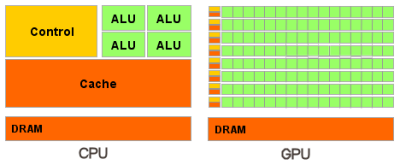
\includegraphics[width=0.8\linewidth]{img/cpu_vs_gpu.png}
\caption{Различие в устройстве CPU и GPU. DRAM --- Оперативная память, Cache --- память процессора для часто используемых операций, Control --- управляющий блок процессора, ALU --- Арифметико-логическое устройство.}
\label{ris:gpucpu}
\end{center}
\end{figure}

Параллельные вычисления на GPU начали активно развиваться с появлением шейдеров --- специальных программ предназначенных для работы на GPU. Тогда же появился компилятор языка Brook --- BrookGPU. BrookGPU облегчал программистам работу с шейдерами. Компилятор обрабатывал файлы с расширением .br и C++ программами давая на выходе скомпилированную программу работающую через DirectX или OpenGL.

Компании Nvidia и ATI увидели возможный потенциал BrookGPU и начали разрабатывать свои аналогичные проекты. Таким образом у Nvidia появился проект CUDA (Compute Unified Device Architecture), а у ATI --- CTM (Close-to-the-Metal) который был началом для AMD FireStream.

\subsection {Nvidia CUDA}

В основе программного интерфейса CUDA лежит расширенный язык Си. Для трансляции текста программы в исполняемые файлы используется компилятор nvcc, созданный на основе открытого компилятора Open64.

Обычная процедура работы с GPU выглядит следующим образом: блок геометрии вычисляет треугольники, блок растеризации вычисляет пиксели которые в дальнейшем будут отображены на экране (Рис.~\ref{ris:process}).

\begin{figure}[ht!]
\begin{center}
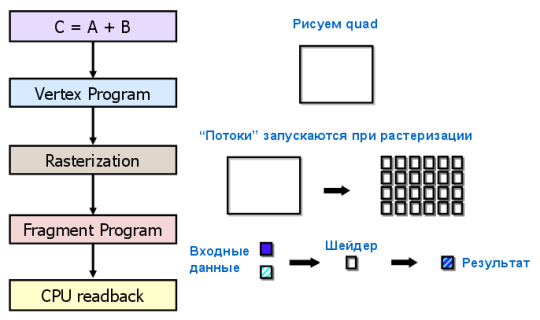
\includegraphics[width=0.5\linewidth]{img/pipeline2.png}
\caption{Обычная процедура обработки фигуры в видеокарте}
\label{ris:process}
\end{center}
\end{figure}

Поэтому использование GPGPU являлось достаточно трудоёмким процессом. Ранние методы работы с графическим процессором были нетривиальными приёмами вследствии чего были крайне неудобными. Данные представлялись изображениями (текстурами), а алгоритмы --- процессами растеризации.

CUDA представляла ряд удобств, вместо непосредственной работы с GPU:

\begin{itemize}
  \item{интерфейс программирования приложений CUDA основан на стандартном языке программирования Си с расширениями, что упрощает процесс изучения и внедрения архитектуры CUDA;}
\item{более эффективная передача данных между системной и видеопамятью;}
\item{отсутствие необходимости в графических API с избыточностью и накладными расходами;}
\item{линейная адресация памяти, и gather и scatter, возможность записи по произвольным адресам;}
\item{аппаратная поддержка целочисленных и битовых операций.}
\end{itemize}

Основные недостатки CUDA:

\begin{itemize}
\item{отсутствие поддержки рекурсии для выполняемых функций;}
\item{минимальная ширина блока в 32 потока;}
\item{закрытая архитектура CUDA, принадлежащая Nvidia.}
\end{itemize}

При написании использовался материал из \cite{nvidiacuda}.

\subsection{AMD FireStream}

Хотя цели видеокарт что у ATI, что у Nvidia одни и те же, но подходы к внутренней архитектуре всё же различаются. В первую очередь это касается основной вычислительной единицы: у Nvidia блок вычисления называется ``warp'' и состоит из 32-х нитей, у ATI блок называется ``wave front'' и состоит из 64-х нитей. Но данное различие не принципиально, практически любую программу для вычисления на GPU можно переписать для использования другого количества нитей. Конечно, может наблюдаться либо падение, либо увеличение производительности, но программа всё же будет работать.

Одно из важных отличий AMD --- это применение технологии ``VLIW'' --- Very Long Instruction Word (Рис.~\ref{ris:ati}). В графических процессорах Nvidia используются простые скалярные инструкции для работы со скалярными регистрами. В архитектуре ATI задействованы 128 битные векторные регистры. Условно назовём компоненты регистра $A$ как $a_1$, $a_2$, $a_3$ и $a_4$; а у регистра $B$ как $b_1$, $b_2$, $b_3$ и $b_4$. Тогда за один такт оказывается возможным вычислить число $a_1 \times b_1 + a_2 \times b_2 + a_3 \times b_3 + a_4 \times b_4$ или двумерный вектор $(a_1 \times b_1 + a_2 \times b_2, a_3 \times b_3 + a_4 \times b_4)$.

Производительность операций на видеокартах ATI при работе над числами одинарной точности достигает нескольких терафлопов благодаря векторным инструкциям.

Также один векторный регистр можно использовать для хранения одного числа двойной точности --- double. В этом случае можно сложить два double числа или умножить два числа, или умножить два числа и сложить с третьим за одну инструкцию. Отсюда при работе над double скорость падает в пять раз чем по сравнению с float. 

\begin{figure}[ht!]
\begin{center}
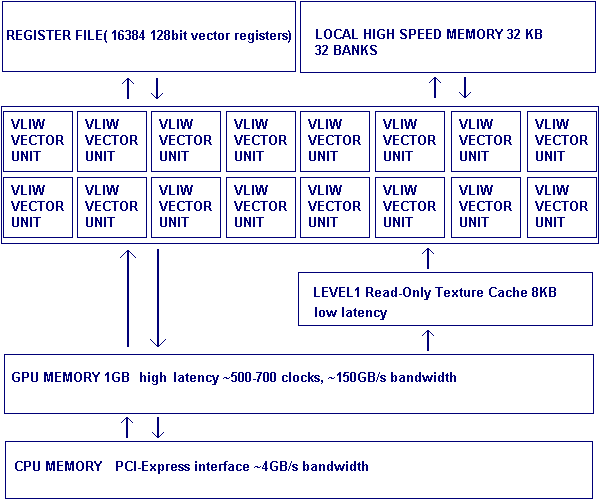
\includegraphics[width=0.8\linewidth]{img/radeon1.png}
\caption{Условная схема работы видеокарт ATI. На рисунке только один минипроцессор из нескольких параллельно работающих.}
\label{ris:ati}
\end{center}
\end{figure}

Ещё одним отличием подхода ATI от Nvidia является использование особого формата расположения инструкций в двоичной коде программы (Табл.~\ref{table:instructions}). У ATI инструкции расположены не традиционно (по тексту исходного кода программы), а секционно.

Прежде всего идёт секция с набором инструкций условных переходов, в них содержатся ссылки на секции арифметических инструкций не содержащих переходов. В секциях с арифметическими операциями (VLIW bundles --- связки VLIW-инструкций) содержатся только арифметические инструкции над данными из регистров и/или локальной памяти. Таким образом становится проще управлять потоком инструкций и доставлять их к устройствам-исполнителям. Кроме того имеются секции для инструкций обращения к памяти.

\begin{table}
\begin{center}
\begin{tabular}{|c|c|c|c|c|}
\hline
\multicolumn{5}{|c|}{Секции инструкций условных переходов} \\
\hline
Секция 0 & Ветвление 0 & \multicolumn{3}{|p{7cm}|}{Ссылка на секцию 3 непрерывных арифметических инструкций} \\ \hline
Секция 1 & Ветвление 1 & \multicolumn{3}{|p{7cm}|}{Ссылка на секцию 4} \\ \hline
Секция 2 & Ветвление 2 & \multicolumn{3}{|p{7cm}|}{Ссылка на секцию 5} \\ \hline
\multicolumn{5}{|c|}{Секции непрерывных арифметических инструкций} \\ \hline
Секция 3 & VLIW 0 & VLIW 1 & VLIW 2 & VLIW 3 \\ \hline
Секция 4 & VLIW 4 & VLIW 5 & & \\ \hline
Секция 5 & VLIW 6 & VLIW 7 & VLIW 8 & VLIW 9 \\ \hline
\end{tabular}
\end{center}
\caption {Схема разбивки программы в архитектуре видеокарт ATI}
\label{table:instructions}
\end{table}

Также существует различие в кэше L1-L2 для видеокарт Nvidia и ATI. Размеры кэша в среднем одинаковы, но существенно различаются время доступа к данным. Задержка доступа к данным у Nvidia несколько больше, и текстурные кэши позволяют сократить загрузку шины памяти, но не ускоряют доступ. У ATI задержка текстурного кэша меньше, но выше задержка локальной памяти минипроцессоров. Для быстрого перемножения матриц у Nvidia лучше использовать локальную память и загружать матрицу поблочно, в случае с AMD лучше использовать быстрый текстурный кэш и читать элементы матрицы по мере необходимости.

Для тех видов задач, которые подходят под идеологию GPU, в частности задачи векторной природы (например, умножение матриц), видеокарты AMD показывают близкую к теоретической производительность. Особенно на задачах с одинарной точностью.

Поэтому архитектура AMD более подходит для научных, профессиональных задач. Для полностью векторных задач, например в задаче параллельного подбора ключей видеокарты AMD в несколько раз опережают Nvidia и в несколько десятков раз быстрее CPU.

В целом идея AMD в том, что графический процессор должен дополнять центральный процессор компьютера выступая в роли своеобразного параллельного сопроцессора для векторных задач.

При написании раздела использовался материал из \cite{amd}.
